\documentclass[article,nojss,shortnames]{jss}\usepackage[]{graphicx}\usepackage[]{color}
% maxwidth is the original width if it is less than linewidth
% otherwise use linewidth (to make sure the graphics do not exceed the margin)
\makeatletter
\def\maxwidth{ %
  \ifdim\Gin@nat@width>\linewidth
    \linewidth
  \else
    \Gin@nat@width
  \fi
}
\makeatother





%% packages
\usepackage{thumbpdf}
\usepackage{amsfonts,amstext,amsmath,amssymb,amsthm}
\usepackage{accents}
\usepackage{color}
\usepackage{rotating}
\usepackage{verbatim}
\usepackage[utf8]{inputenc}
\usepackage{booktabs}
\usepackage{tikz}
\usepackage{multirow}
%% need no \usepackage{Sweave.sty}
%%\usepackage[nolists]{endfloat}

\newcommand{\cmd}[1]{\texttt{#1()}}



\newcommand{\TODO}[1]{{\color{red} #1}}

% File with math commands etc.
\usepackage{bbm}
\usepackage{accents}

\newcommand{\1}{\mathbbm{1}}

%%% mlt
%% rv
\newcommand{\rZ}{Z}
\newcommand{\rY}{Y}
\newcommand{\rX}{\mX}
\newcommand{\rS}{\mS}
\newcommand{\rs}{\svec}
\newcommand{\rz}{z}
\newcommand{\ry}{y}
\newcommand{\rx}{\xvec}
\newcommand{\erx}{x}
%% sigma algebra
\newcommand{\sA}{\mathfrak{A}}
\newcommand{\sAZ}{\mathfrak{B}}
\newcommand{\sAY}{\mathfrak{C}}
\newcommand{\esA}{A}
\newcommand{\esAZ}{B}
\newcommand{\esAY}{C}
%% sample spaces
\newcommand{\sam}{\Omega}
\newcommand{\samZ}{\RR}
\newcommand{\samY}{\Xi}
\newcommand{\samX}{\chi}
%% measureable spaces
\newcommand{\ms}{(\sam, \sA)}
\newcommand{\msZ}{(\samZ, \sAZ)}
\newcommand{\msY}{(\samY, \sAY)}
%% probability spaces
\newcommand{\ps}{(\sam, \sA, \Prob)}
\newcommand{\psZ}{(\samZ, \sAZ, \Prob_\rZ)}
\newcommand{\psY}{(\samY, \sAY, \Prob_\rY)}
%% distributions
\newcommand{\pZ}{F_\rZ}
\newcommand{\pY}{F_\rY}
\newcommand{\hatpY}{\hat{F}_{\rY,N}}
\newcommand{\hatpYx}{\hat{F}_{\rY | \rX = \rx, N}}
\newcommand{\pN}{\Phi}
\newcommand{\pSL}{F_{\SL}}
\newcommand{\pMEV}{F_{\MEV}}
\newcommand{\pGumbel}{F_{\text{Gumbel}}}
\newcommand{\pSW}{F_{\SW}}
\newcommand{\pYx}{F_{\rY | \rX = \rx}}
\newcommand{\pYA}{F_{\rY | \rX = A}}
\newcommand{\pYB}{F_{\rY | \rX = B}}
\newcommand{\qZ}{F^{-1}_\rZ}
\newcommand{\qY}{F^{-1}_\rY}
\newcommand{\dZ}{f_\rZ}
\newcommand{\dY}{f_\rY}
\newcommand{\hatdY}{\hat{f}_{\rY, N}}
\newcommand{\dYx}{f_{\rY | \rX = \rx}}
\newcommand{\hazY}{\lambda_{\rY}}
\newcommand{\HazY}{\Lambda_{\rY}}
\newcommand{\hathazY}{\hat{\lambda}_{\rY, N}}
\newcommand{\hatHazY}{\hat{\Lambda}_{\rY, N}}
%% measures
\newcommand{\measureY}{\mu}
\newcommand{\lebesgue}{\mu_L}
\newcommand{\counting}{\mu_C}
%% trafo
\newcommand{\g}{g}
\newcommand{\h}{h}
\newcommand{\s}{\svec}
\newcommand{\hY}{h_\rY}
\newcommand{\hx}{h_\rx}
\newcommand{\hs}{\mathcal{H}}
\newcommand{\basisy}{\avec}
\newcommand{\bern}[1]{\avec_{\text{Bs},#1}}
\newcommand{\bernx}[1]{\bvec_{\text{Bs},#1}}
\newcommand{\basisx}{\bvec}
\newcommand{\basisyx}{\cvec}
\newcommand{\m}{m}
\newcommand{\lik}{\mathcal{L}}
\newcommand{\parm}{\varthetavec}
\newcommand{\eparm}{\vartheta}
\newcommand{\dimparm}{P}
\newcommand{\dimparmx}{Q}
\newcommand{\shiftparm}{\betavec}
\newcommand{\baseparm}{\alphavec}
\newcommand{\eshiftparm}{\beta}

\newcommand{\ie}{\textit{i.e.}~}
\newcommand{\eg}{\textit{e.g.}~}

\newcommand{\prob}{\mathbb{P}}
\newcommand{\Ex}{\mathbb{E}}
\newcommand{\RR}{\mathbb{R}}
\newcommand{\eps}{\varepsilon}
\newcommand{\prodname}{tensor }
\newcommand{\Null}{\mathbf{0}}
\newcommand{\FI}{\mF}

\usepackage{dsfont}
\newcommand{\I}{\mathds{1}}

\newcommand{\given}{\rvert}

\def \dsP {\text{$\mathds{P}$}}
\def \dsE {\text{$\mathds{E}$}}
\def \dsR {\text{$\mathds{R}$}}
\def \dsN {\text{$\mathds{N}$}}


% Math Operators
 \DeclareMathOperator{\CE}{CE}
 \DeclareMathOperator{\CV}{CV}
 \DeclareMathOperator{\logit}{logit}
 \DeclareMathOperator{\expit}{expit}
 \DeclareMathOperator{\LRT}{LRT}
 \DeclareMathOperator{\RLRT}{RLRT}
 \DeclareMathOperator{\Cov}{Cov}
 \DeclareMathOperator{\Cor}{Cor}
 \DeclareMathOperator{\Var}{Var}
 \DeclareMathOperator{\EW}{\dsE}
 \DeclareMathOperator{\D}{D}
 \DeclareMathOperator{\Bias}{Bias}
 \DeclareMathOperator{\MSE}{MSE}
 \DeclareMathOperator{\PLS}{PLS}
 \DeclareMathOperator{\rank}{rank}
 \DeclareMathOperator{\ncol}{ncol}
 \DeclareMathOperator{\pen}{pen}
 \DeclareMathOperator{\const}{const}
 \DeclareMathOperator{\diag}{diag}
 \DeclareMathOperator{\blockdiag}{blockdiag}
 \DeclareMathOperator{\df}{df}
 \DeclareMathOperator{\trace}{tr}
 \DeclareMathOperator{\iid}{i.i.d.}
 \DeclareMathOperator{\ind}{ind.}
 \DeclareMathOperator{\obs}{obs}
 \DeclareMathOperator{\acos}{acos}
 \DeclareMathOperator{\spat}{spat}
 \DeclareMathOperator{\fix}{{fix}}
 \DeclareMathOperator{\ran}{{ran}}
 \DeclareMathOperator*{\argmin}{{arg\,min}}
 \DeclareMathOperator*{\argmax}{{arg\,max}}
 \DeclareMathOperator{\BIC}{{BIC}}
 \DeclareMathOperator{\DIC}{{DIC}}
 \DeclareMathOperator{\AIC}{{AIC}}
 \DeclareMathOperator{\mAIC}{{mAIC}}
 \DeclareMathOperator{\cAIC}{{cAIC}}
 \DeclareMathOperator{\cloglog}{cloglog}
 \DeclareMathOperator{\softmax}{softmax}
% Distributions

 \DeclareMathOperator{\ND}{N}
 \DeclareMathOperator{\TND}{TN}
 \DeclareMathOperator{\UD}{U}
 \DeclareMathOperator{\GaD}{Ga}
 \DeclareMathOperator{\tD}{t}
 \DeclareMathOperator{\IGD}{IG}
 \DeclareMathOperator{\IWD}{IW}
 \DeclareMathOperator{\PoD}{Po}
 \DeclareMathOperator{\ExpD}{Exp}
 \DeclareMathOperator{\LapD}{Lap}
 \DeclareMathOperator{\MuD}{Mu}
 \DeclareMathOperator{\DirD}{Dir}
 \DeclareMathOperator{\PDD}{PD}
 \DeclareMathOperator{\BeD}{Be}
 \DeclareMathOperator{\BD}{B}
 \DeclareMathOperator{\DPD}{DP}
 \DeclareMathOperator{\KSD}{KS}
 \DeclareMathOperator{\SL}{SL}
 \DeclareMathOperator{\MEV}{MEV}
 \DeclareMathOperator{\SW}{SW}
 \DeclareMathOperator{\Chi1}{\chi^2_1}



% Boldface vectors and matrices

% \def \avec {\text{\boldmath$a$}}    \def \mA {\text{\boldmath$A$}}
% \def \bvec {\text{\boldmath$b$}}    \def \mB {\text{\boldmath$B$}}
% \def \cvec {\text{\boldmath$c$}}    \def \mC {\text{\boldmath$C$}}
% \def \dvec {\text{\boldmath$d$}}    \def \mD {\text{\boldmath$D$}}
% \def \evec {\text{\boldmath$e$}}    \def \mE {\text{\boldmath$E$}}
% \def \fvec {\text{\boldmath$f$}}    \def \mF {\text{\boldmath$F$}}
% \def \gvec {\text{\boldmath$g$}}    \def \mG {\text{\boldmath$G$}}
% \def \hvec {\text{\boldmath$h$}}    \def \mH {\text{\boldmath$H$}}
% \def \ivec {\text{\boldmath$i$}}    \def \mI {\text{\boldmath$I$}}
% \def \jvec {\text{\boldmath$j$}}    \def \mJ {\text{\boldmath$J$}}
% \def \kvec {\text{\boldmath$k$}}    \def \mK {\text{\boldmath$K$}}
% \def \lvec {\text{\boldmath$l$}}    \def \mL {\text{\boldmath$L$}}
% \def \mvec {\text{\boldmath$m$}}    \def \mM {\text{\boldmath$M$}}
% \def \nvec {\text{\boldmath$n$}}    \def \mN {\text{\boldmath$N$}}
% \def \ovec {\text{\boldmath$o$}}    \def \mO {\text{\boldmath$O$}}
% \def \pvec {\text{\boldmath$p$}}    \def \mP {\text{\boldmath$P$}}
% \def \qvec {\text{\boldmath$q$}}    \def \mQ {\text{\boldmath$Q$}}
% \def \rvec {\text{\boldmath$r$}}    \def \mR {\text{\boldmath$R$}}
% \def \svec {\text{\boldmath$s$}}    \def \mS {\text{\boldmath$S$}}
% \def \tvec {\text{\boldmath$t$}}    \def \mT {\text{\boldmath$T$}}
% \def \uvec {\text{\boldmath$u$}}    \def \mU {\text{\boldmath$U$}}
% \def \vvec {\text{\boldmath$v$}}    \def \mV {\text{\boldmath$V$}}
% \def \wvec {\text{\boldmath$w$}}    \def \mW {\text{\boldmath$W$}}
% \def \xvec {\text{\boldmath$x$}}    \def \mX {\text{\boldmath$X$}}
% \def \yvec {\text{\boldmath$y$}}    \def \mY {\text{\boldmath$Y$}}
% \def \zvec {\text{\boldmath$z$}}    \def \mZ {\text{\boldmath$Z$}}

\def \avec {\boldsymbol a}   \def \mA {\boldsymbol A}
\def \bvec {\boldsymbol b}   \def \mB {\boldsymbol B}
\def \cvec {\boldsymbol c}   \def \mC {\boldsymbol C}
\def \dvec {\boldsymbol d}   \def \mD {\boldsymbol D}
\def \evec {\boldsymbol e}   \def \mE {\boldsymbol E}
\def \fvec {\boldsymbol f}   \def \mF {\boldsymbol F}
\def \gvec {\boldsymbol g}   \def \mG {\boldsymbol G}
\def \hvec {\boldsymbol h}   \def \mH {\boldsymbol H}
\def \ivec {\boldsymbol i}   \def \mI {\boldsymbol I}
\def \jvec {\boldsymbol j}   \def \mJ {\boldsymbol J}
\def \kvec {\boldsymbol k}   \def \mK {\boldsymbol K}
\def \lvec {\boldsymbol l}   \def \mL {\boldsymbol L}
\def \mvec {\boldsymbol m}   \def \mM {\boldsymbol M}
\def \nvec {\boldsymbol n}   \def \mN {\boldsymbol N}
\def \ovec {\boldsymbol o}   \def \mO {\boldsymbol O}
\def \pvec {\boldsymbol p}   \def \mP {\boldsymbol P}
\def \qvec {\boldsymbol q}   \def \mQ {\boldsymbol Q}
\def \rvec {\boldsymbol r}   \def \mR {\boldsymbol R}
\def \svec {\boldsymbol s}   \def \mS {\boldsymbol S}
\def \tvec {\boldsymbol t}   \def \mT {\boldsymbol T}
\def \uvec {\boldsymbol u}   \def \mU {\boldsymbol U}
\def \vvec {\boldsymbol v}   \def \mV {\boldsymbol V}
\def \wvec {\boldsymbol w}   \def \mW {\boldsymbol W}
\def \xvec {\boldsymbol x}   \def \mX {\boldsymbol X}
\def \yvec {\boldsymbol y}   \def \mY {\boldsymbol Y}
\def \zvec {\boldsymbol z}   \def \mZ {\boldsymbol Z}

 \def \calA {\mathcal A}
 \def \calB {\mathcal B}
 \def \calC {\mathcal C}
 \def \calD {\mathcal D}
 \def \calE {\mathcal E}
 \def \calF {\mathcal F}
 \def \calG {\mathcal G}
 \def \calH {\mathcal H}
 \def \calI {\mathcal I}
 \def \calJ {\mathcal J}
 \def \calK {\mathcal K}
 \def \calL {\mathcal L}
 \def \calM {\mathcal M}
 \def \calN {\mathcal N}
 \def \calO {\mathcal O}
 \def \calP {\mathcal P}
 \def \calQ {\mathcal Q}
 \def \calR {\mathcal R}
 \def \calS {\mathcal S}
 \def \calT {\mathcal T}
 \def \calU {\mathcal U}
 \def \calV {\mathcal V}
 \def \calW {\mathcal W}
 \def \calX {\mathcal X}
 \def \calY {\mathcal Y}
 \def \calZ {\mathcal Z}

\def \ahatvec {\text{\boldmath$\hat a$}}    \def \mhatA {\text{\boldmath$\hat A$}}
\def \bhatvec {\text{\boldmath$\hat b$}}    \def \mhatB {\text{\boldmath$\hat B$}}
\def \chatvec {\text{\boldmath$\hat c$}}    \def \mhatC {\text{\boldmath$\hat C$}}
\def \dhatvec {\text{\boldmath$\hat d$}}    \def \mhatD {\text{\boldmath$\hat D$}}
\def \ehatvec {\text{\boldmath$\hat e$}}    \def \mhatE {\text{\boldmath$\hat E$}}
\def \fhatvec {\text{\boldmath$\hat f$}}    \def \mhatF {\text{\boldmath$\hat F$}}
\def \ghatvec {\text{\boldmath$\hat g$}}    \def \mhatG {\text{\boldmath$\hat G$}}
\def \hhatvec {\text{\boldmath$\hat h$}}    \def \mhatH {\text{\boldmath$\hat H$}}
\def \ihatvec {\text{\boldmath$\hat i$}}    \def \mhatI {\text{\boldmath$\hat I$}}
\def \jhatvec {\text{\boldmath$\hat j$}}    \def \mhatJ {\text{\boldmath$\hat J$}}
\def \khatvec {\text{\boldmath$\hat k$}}    \def \mhatK {\text{\boldmath$\hat K$}}
\def \lhatvec {\text{\boldmath$\hat l$}}    \def \mhatL {\text{\boldmath$\hat L$}}
\def \mhatvec {\text{\boldmath$\hat m$}}    \def \mhatM {\text{\boldmath$\hat M$}}
\def \nhatvec {\text{\boldmath$\hat n$}}    \def \mhatN {\text{\boldmath$\hat N$}}
\def \ohatvec {\text{\boldmath$\hat o$}}    \def \mhatO {\text{\boldmath$\hat O$}}
\def \phatvec {\text{\boldmath$\hat p$}}    \def \mhatP {\text{\boldmath$\hat P$}}
\def \qhatvec {\text{\boldmath$\hat q$}}    \def \mhatQ {\text{\boldmath$\hat Q$}}
\def \rhatvec {\text{\boldmath$\hat r$}}    \def \mhatR {\text{\boldmath$\hat R$}}
\def \shatvec {\text{\boldmath$\hat s$}}    \def \mhatS {\text{\boldmath$\hat S$}}
\def \thatvec {\text{\boldmath$\hat t$}}    \def \mhatT {\text{\boldmath$\hat T$}}
\def \uhatvec {\text{\boldmath$\hat u$}}    \def \mhatU {\text{\boldmath$\hat U$}}
\def \vhatvec {\text{\boldmath$\hat v$}}    \def \mhatV {\text{\boldmath$\hat V$}}
\def \whatvec {\text{\boldmath$\hat w$}}    \def \mhatW {\text{\boldmath$\hat W$}}
\def \xhatvec {\text{\boldmath$\hat x$}}    \def \mhatX {\text{\boldmath$\hat X$}}
\def \yhatvec {\text{\boldmath$\hat y$}}    \def \mhatY {\text{\boldmath$\hat Y$}}
\def \zhatvec {\text{\boldmath$\hat z$}}    \def \mhatZ {\text{\boldmath$\hat Z$}}


\def \atildevec {\text{\boldmath$\tilde a$}}    \def \mtildeA {\text{\boldmath$\tilde A$}}
\def \btildevec {\text{\boldmath$\tilde b$}}    \def \mtildeB {\text{\boldmath$\tilde B$}}
\def \ctildevec {\text{\boldmath$\tilde c$}}    \def \mtildeC {\text{\boldmath$\tilde C$}}
\def \dtildevec {\text{\boldmath$\tilde d$}}    \def \mtildeD {\text{\boldmath$\tilde D$}}
\def \etildevec {\text{\boldmath$\tilde e$}}    \def \mtildeE {\text{\boldmath$\tilde E$}}
\def \ftildevec {\text{\boldmath$\tilde f$}}    \def \mtildeF {\text{\boldmath$\tilde F$}}
\def \gtildevec {\text{\boldmath$\tilde g$}}    \def \mtildeG {\text{\boldmath$\tilde G$}}
\def \htildevec {\text{\boldmath$\tilde h$}}    \def \mtildeH {\text{\boldmath$\tilde H$}}
\def \itildevec {\text{\boldmath$\tilde i$}}    \def \mtildeI {\text{\boldmath$\tilde I$}}
\def \jtildevec {\text{\boldmath$\tilde j$}}    \def \mtildeJ {\text{\boldmath$\tilde J$}}
\def \ktildevec {\text{\boldmath$\tilde k$}}    \def \mtildeK {\text{\boldmath$\tilde K$}}
\def \ltildevec {\text{\boldmath$\tilde l$}}    \def \mtildeL {\text{\boldmath$\tilde L$}}
\def \mtildevec {\text{\boldmath$\tilde m$}}    \def \mtildeM {\text{\boldmath$\tilde M$}}
\def \ntildevec {\text{\boldmath$\tilde n$}}    \def \mtildeN {\text{\boldmath$\tilde N$}}
\def \otildevec {\text{\boldmath$\tilde o$}}    \def \mtildeO {\text{\boldmath$\tilde O$}}
\def \ptildevec {\text{\boldmath$\tilde p$}}    \def \mtildeP {\text{\boldmath$\tilde P$}}
\def \qtildevec {\text{\boldmath$\tilde q$}}    \def \mtildeQ {\text{\boldmath$\tilde Q$}}
\def \rtildevec {\text{\boldmath$\tilde r$}}    \def \mtildeR {\text{\boldmath$\tilde R$}}
\def \stildevec {\text{\boldmath$\tilde s$}}    \def \mtildeS {\text{\boldmath$\tilde S$}}
\def \ttildevec {\text{\boldmath$\tilde t$}}    \def \mtildeT {\text{\boldmath$\tilde T$}}
\def \utildevec {\text{\boldmath$\tilde u$}}    \def \mtildeU {\text{\boldmath$\tilde U$}}
\def \vtildevec {\text{\boldmath$\tilde v$}}    \def \mtildeV {\text{\boldmath$\tilde V$}}
\def \wtildevec {\text{\boldmath$\tilde w$}}    \def \mtildeW {\text{\boldmath$\tilde W$}}
\def \xtildevec {\text{\boldmath$\tilde x$}}    \def \mtildeX {\text{\boldmath$\tilde X$}}
\def \ytildevec {\text{\boldmath$\tilde y$}}    \def \mtildeY {\text{\boldmath$\tilde Y$}}
\def \ztildevec {\text{\boldmath$\tilde z$}}    \def \mtildeZ {\text{\boldmath$\tilde Z$}}

\def \alphavec        {\text{\boldmath$\alpha$}}
\def \betavec         {\text{\boldmath$\beta$}}
\def \gammavec        {\text{\boldmath$\gamma$}}
\def \deltavec        {\text{\boldmath$\delta$}}
\def \epsilonvec      {\text{\boldmath$\epsilon$}}
\def \varepsilonvec   {\text{\boldmath$\varepsilon$}}
\def \zetavec         {\text{\boldmath$\zeta$}}
\def \etavec          {\text{\boldmath$\eta$}}
\def \thetavec        {\text{\boldmath$\theta$}}
\def \varthetavec     {\text{\boldmath$\vartheta$}}
\def \iotavec         {\text{\boldmath$\iota$}}
\def \kappavec        {\text{\boldmath$\kappa$}}
\def \lambdavec       {\text{\boldmath$\lambda$}}
\def \muvec           {\text{\boldmath$\mu$}}
\def \nuvec           {\text{\boldmath$\nu$}}
\def \xivec           {\text{\boldmath$\xi$}}
\def \pivec           {\text{\boldmath$\pi$}}
\def \varpivec        {\text{\boldmath$\varpi$}}
\def \rhovec          {\text{\boldmath$\rho$}}
\def \varrhovec       {\text{\boldmath$\varrho$}}
\def \sigmavec        {\text{\boldmath$\sigma$}}
\def \varsigmavec     {\text{\boldmath$\varsigma$}}
\def \tauvec          {\text{\boldmath$\tau$}}
\def \upsilonvec      {\text{\boldmath$\upsilon$}}
\def \phivec          {\text{\boldmath$\phi$}}
\def \varphivec       {\text{\boldmath$\varphi$}}
\def \psivec          {\text{\boldmath$\psi$}}
\def \chivec          {\text{\boldmath$\chi$}}
\def \omegavec        {\text{\boldmath$\omega$}}

\def \alphahatvec        {\text{\boldmath$\hat \alpha$}}
\def \betahatvec         {\text{\boldmath$\hat \beta$}}
\def \gammahatvec        {\text{\boldmath$\hat \gamma$}}
\def \deltahatvec        {\text{\boldmath$\hat \delta$}}
\def \epsilonhatvec      {\text{\boldmath$\hat \epsilon$}}
\def \varepsilonhatvec   {\text{\boldmath$\hat \varepsilon$}}
\def \zetahatvec         {\text{\boldmath$\hat \zeta$}}
\def \etahatvec          {\text{\boldmath$\hat \eta$}}
\def \thetahatvec        {\text{\boldmath$\hat \theta$}}
\def \varthetahatvec     {\text{\boldmath$\hat \vartheta$}}
\def \iotahatvec         {\text{\boldmath$\hat \iota$}}
\def \kappahatvec        {\text{\boldmath$\hat \kappa$}}
\def \lambdahatvec       {\text{\boldmath$\hat \lambda$}}
\def \muhatvec           {\text{\boldmath$\hat \mu$}}
\def \nuhatvec           {\text{\boldmath$\hat \nu$}}
\def \xihatvec           {\text{\boldmath$\hat \xi$}}
\def \pihatvec           {\text{\boldmath$\hat \pi$}}
\def \varpihatvec        {\text{\boldmath$\hat \varpi$}}
\def \rhohatvec          {\text{\boldmath$\hat \rho$}}
\def \varrhohatvec       {\text{\boldmath$\hat \varrho$}}
\def \sigmahatvec        {\text{\boldmath$\hat \sigma$}}
\def \varsigmahatvec     {\text{\boldmath$\hat \varsigma$}}
\def \tauhatvec          {\text{\boldmath$\hat \tau$}}
\def \upsilonhatvec      {\text{\boldmath$\hat \upsilon$}}
\def \phihatvec          {\text{\boldmath$\hat \phi$}}
\def \varphihatvec       {\text{\boldmath$\hat \varphi$}}
\def \psihatvec          {\text{\boldmath$\hat \psi$}}
\def \chihatvec          {\text{\boldmath$\hat \chi$}}
\def \omegahatvec        {\text{\boldmath$\hat \omega$}}

\def \alphatildevec        {\text{\boldmath$\tilde \alpha$}}
\def \betatildevec         {\text{\boldmath$\tilde \beta$}}
\def \gammatildevec        {\text{\boldmath$\tilde \gamma$}}
\def \deltatildevec        {\text{\boldmath$\tilde \delta$}}
\def \epsilontildevec      {\text{\boldmath$\tilde \epsilon$}}
\def \varepsilontildevec   {\text{\boldmath$\tilde \varepsilon$}}
\def \zetatildevec         {\text{\boldmath$\tilde \zeta$}}
\def \etatildevec          {\text{\boldmath$\tilde \eta$}}
\def \thetatildevec        {\text{\boldmath$\tilde \theta$}}
\def \varthetatildevec     {\text{\boldmath$\tilde \vartheta$}}
\def \iotatildevec         {\text{\boldmath$\tilde \iota$}}
\def \kappatildevec        {\text{\boldmath$\tilde \kappa$}}
\def \lambdatildevec       {\text{\boldmath$\tilde \lambda$}}
\def \mutildevec           {\text{\boldmath$\tilde \mu$}}
\def \nutildevec           {\text{\boldmath$\tilde \nu$}}
\def \xitildevec           {\text{\boldmath$\tilde \xi$}}
\def \pitildevec           {\text{\boldmath$\tilde \pi$}}
\def \varpitildevec        {\text{\boldmath$\tilde \varpi$}}
\def \rhotildevec          {\text{\boldmath$\tilde \rho$}}
\def \varrhotildevec       {\text{\boldmath$\tilde \varrho$}}
\def \sigmatildevec        {\text{\boldmath$\tilde \sigma$}}
\def \varsigmatildevec     {\text{\boldmath$\tilde \varsigma$}}
\def \tautildevec          {\text{\boldmath$\tilde \tau$}}
\def \upsilontildevec      {\text{\boldmath$\tilde \upsilon$}}
\def \phitildevec          {\text{\boldmath$\tilde \phi$}}
\def \varphitildevec       {\text{\boldmath$\tilde \varphi$}}
\def \psitildevec          {\text{\boldmath$\tilde \psi$}}
\def \chitildevec          {\text{\boldmath$\tilde \chi$}}
\def \omegatildevec        {\text{\boldmath$\tilde \omega$}}

\def \B {\mathsf{B}}
\def \bB {\boldsymbol{\B}}
\def \linpred {\rx^\top\shiftparm}

\def \mGamma   {\mathbf{\Gamma}}
\def \mDelta   {\mathbf{\Delta}}
\def \mTheta   {\mathbf{\Theta}}
\def \mLambda  {\mathbf{\Lambda}}
\def \mXi      {\mathbf{\Xi}}
\def \mPi      {\mathbf{\Pi}}
\def \mSigma   {\mathbf{\Sigma}}
\def \mUpsilon {\mathbf{\Upsilon}}
\def \mPhi     {\mathbf{\Phi}}
\def \mPsi     {\mathbf{\Psi}}
\def \mOmega   {\mathbf{\Omega}}

\def \mhatGamma   {\mathbf{\hat \Gamma}}
\def \mhatDelta   {\mathbf{\hat \Delta}}
\def \mhatTheta   {\mathbf{\hat \Theta}}
\def \mhatLambda  {\mathbf{\hat \Lambda}}
\def \mhatXi      {\mathbf{\hat \Xi}}
\def \mhatPi      {\mathbf{\hat \Pi}}
\def \mhatSigma   {\mathbf{\hat \Sigma}}
\def \mhatUpsilon {\mathbf{\hat \Upsilon}}
\def \mhatPhi     {\mathbf{\hat \Phi}}
\def \mhatPsi     {\mathbf{\hat \Psi}}
\def \mhatOmega   {\mathbf{\hat \Omega}}

\def \nullvec {\mathbf{0}}
\def \onevec {\mathbf{1}}

%%% theorems
\newtheorem{lem}{Lemma}
\newtheorem{thm}{Theorem}
\newtheorem{coro}{Corollary}
\newtheorem{defn}{Definition}
\newtheorem{remark}{Remark}

\newcommand{\ubar}[1]{\underaccent{\bar}{#1}}

\theoremstyle{definition}
\newtheorem{exmpl}{Example}

\usepackage{tikz}

\usetikzlibrary{positioning, calc, shapes.geometric, shapes.multipart,
  shapes, arrows.meta, arrows, quotes,
  decorations.markings, external, trees}
\tikzstyle{line} = [draw, -latex']
\tikzstyle{Arrow} = [
        thick,
        decoration={
                markings,
                mark=at position 1 with {
                        \arrow[thick]{latex}
} },
        shorten >= 3pt, preaction = {decorate}
        ]


\renewcommand{\thefootnote}{}

%% code commands
\newcommand{\Rclass}[1]{`\code{#1}'}
%% JSS
\author{Lucas Kook*, Lisa Herzog*, Torsten Hothorn, Oliver D\"urr, Beate Sick}
\Plainauthor{}

\title{Ordinal neural transformation models}
\Plaintitle{Ordinal neural transformation models}
\Shorttitle{\pkg{ontram}}

\Abstract{Model formulations and log-likelihood contributions for the models
used in \pkg{ontram}. Draft for introduction and methods section. Literature review.}

\Keywords{Notation, literature}
\Plainkeywords{Notation, literature}

\Address{}
\IfFileExists{upquote.sty}{\usepackage{upquote}}{}
\begin{document}



%%%%%%%%%%%%%%%%%%%%%%%%%%%%%%%%%%%%%%%%%%%%%%%%%%%%%%%%%%%%%%%%%%%%%%%%%%%%%%%%
\section{Introduction}
%-------------------------------------------------------------------------------

Ordinal regression problems arise for categorical responses with naturally
ordered categories, such as disease gradings. Ordinal regression thus differs from
ordinary multi-class classification problems in that this ordering should be taken
into account when estimating and evaluating the model.
Ordinal regression has been studied extensively in the statistical literature
for more than four decades \citep{mccullagh1980regression, genter1985goodness}.
An ordinal random variable $\rY$ can take values in
$\{\ry_1 < \ry_2 < \dots < \ry_K\}, \; K \geq 2$ and is fully described by
its cumulative distribution function $\prob(\rY \leq \ry_k) = \pY(\ry_k)$, from
which the density function can be retrieved as
$\prob(\rY = \ry_k) = \pY(\ry_k) - \pY(\ry_{k-1}), \; k = 2, \dots, K$.
% Notice, that in this unconditional case the density of an unordered response with
% $K$ categories could look exactly the same when imposing an arbitrary ordering
% on its sample space.
The goal of ordinal regression is now to estimate a conditional distribution
function in a way that takes the ordering of $\rY$ into account. For instance,
adjacent categories should be more similar to each other than categories that
are further apart.
Ordinal regression problems can be viewed as a special case of a more general
class of transformation models
\begin{align} \label{eq:ctm}
  \prob(\rY \leq \ry \given \rx) = F(\h(\ry \given \rx)),
\end{align}
with a discrete transformation function $\h$ with $K - 1$ steps.
Here, the conditional distribution is decomposed into an inverse cumulative link
function $F$ and a non-decreasing conditional transformation function $\h$ and
$\rx$ denotes the explanatory variables such as tabular data or images.
This general formulation of ordinal regression models as transformation models
\citep{hothorn2014conditional, hothorn2018most} encompasses the classic
proportional odds logistic and discrete proportional hazards regression models
\citep{mccullagh1980regression}, and the cumulative probit and Gumbel models
\citep{tutz2011regression}, depending on the choice of $F$ and $\h$.
The various interpretational scales are induced by $F$. For instance, $F = \expit$
allows the interpretation of $\h$ on a log-odds scale \citet{tutz2011regression}.

Cumulative ordinal regression models work by splitting the real number line into
$K$ categories determined by the $K - 1$ intercept terms that are estimated from
the data. The individual likelihood contributions are the probabilities given by
the are under the density of $F$ between two consecutive intercepts
(see Figure~\ref{fig:discrete}).
\begin{figure}
\centering
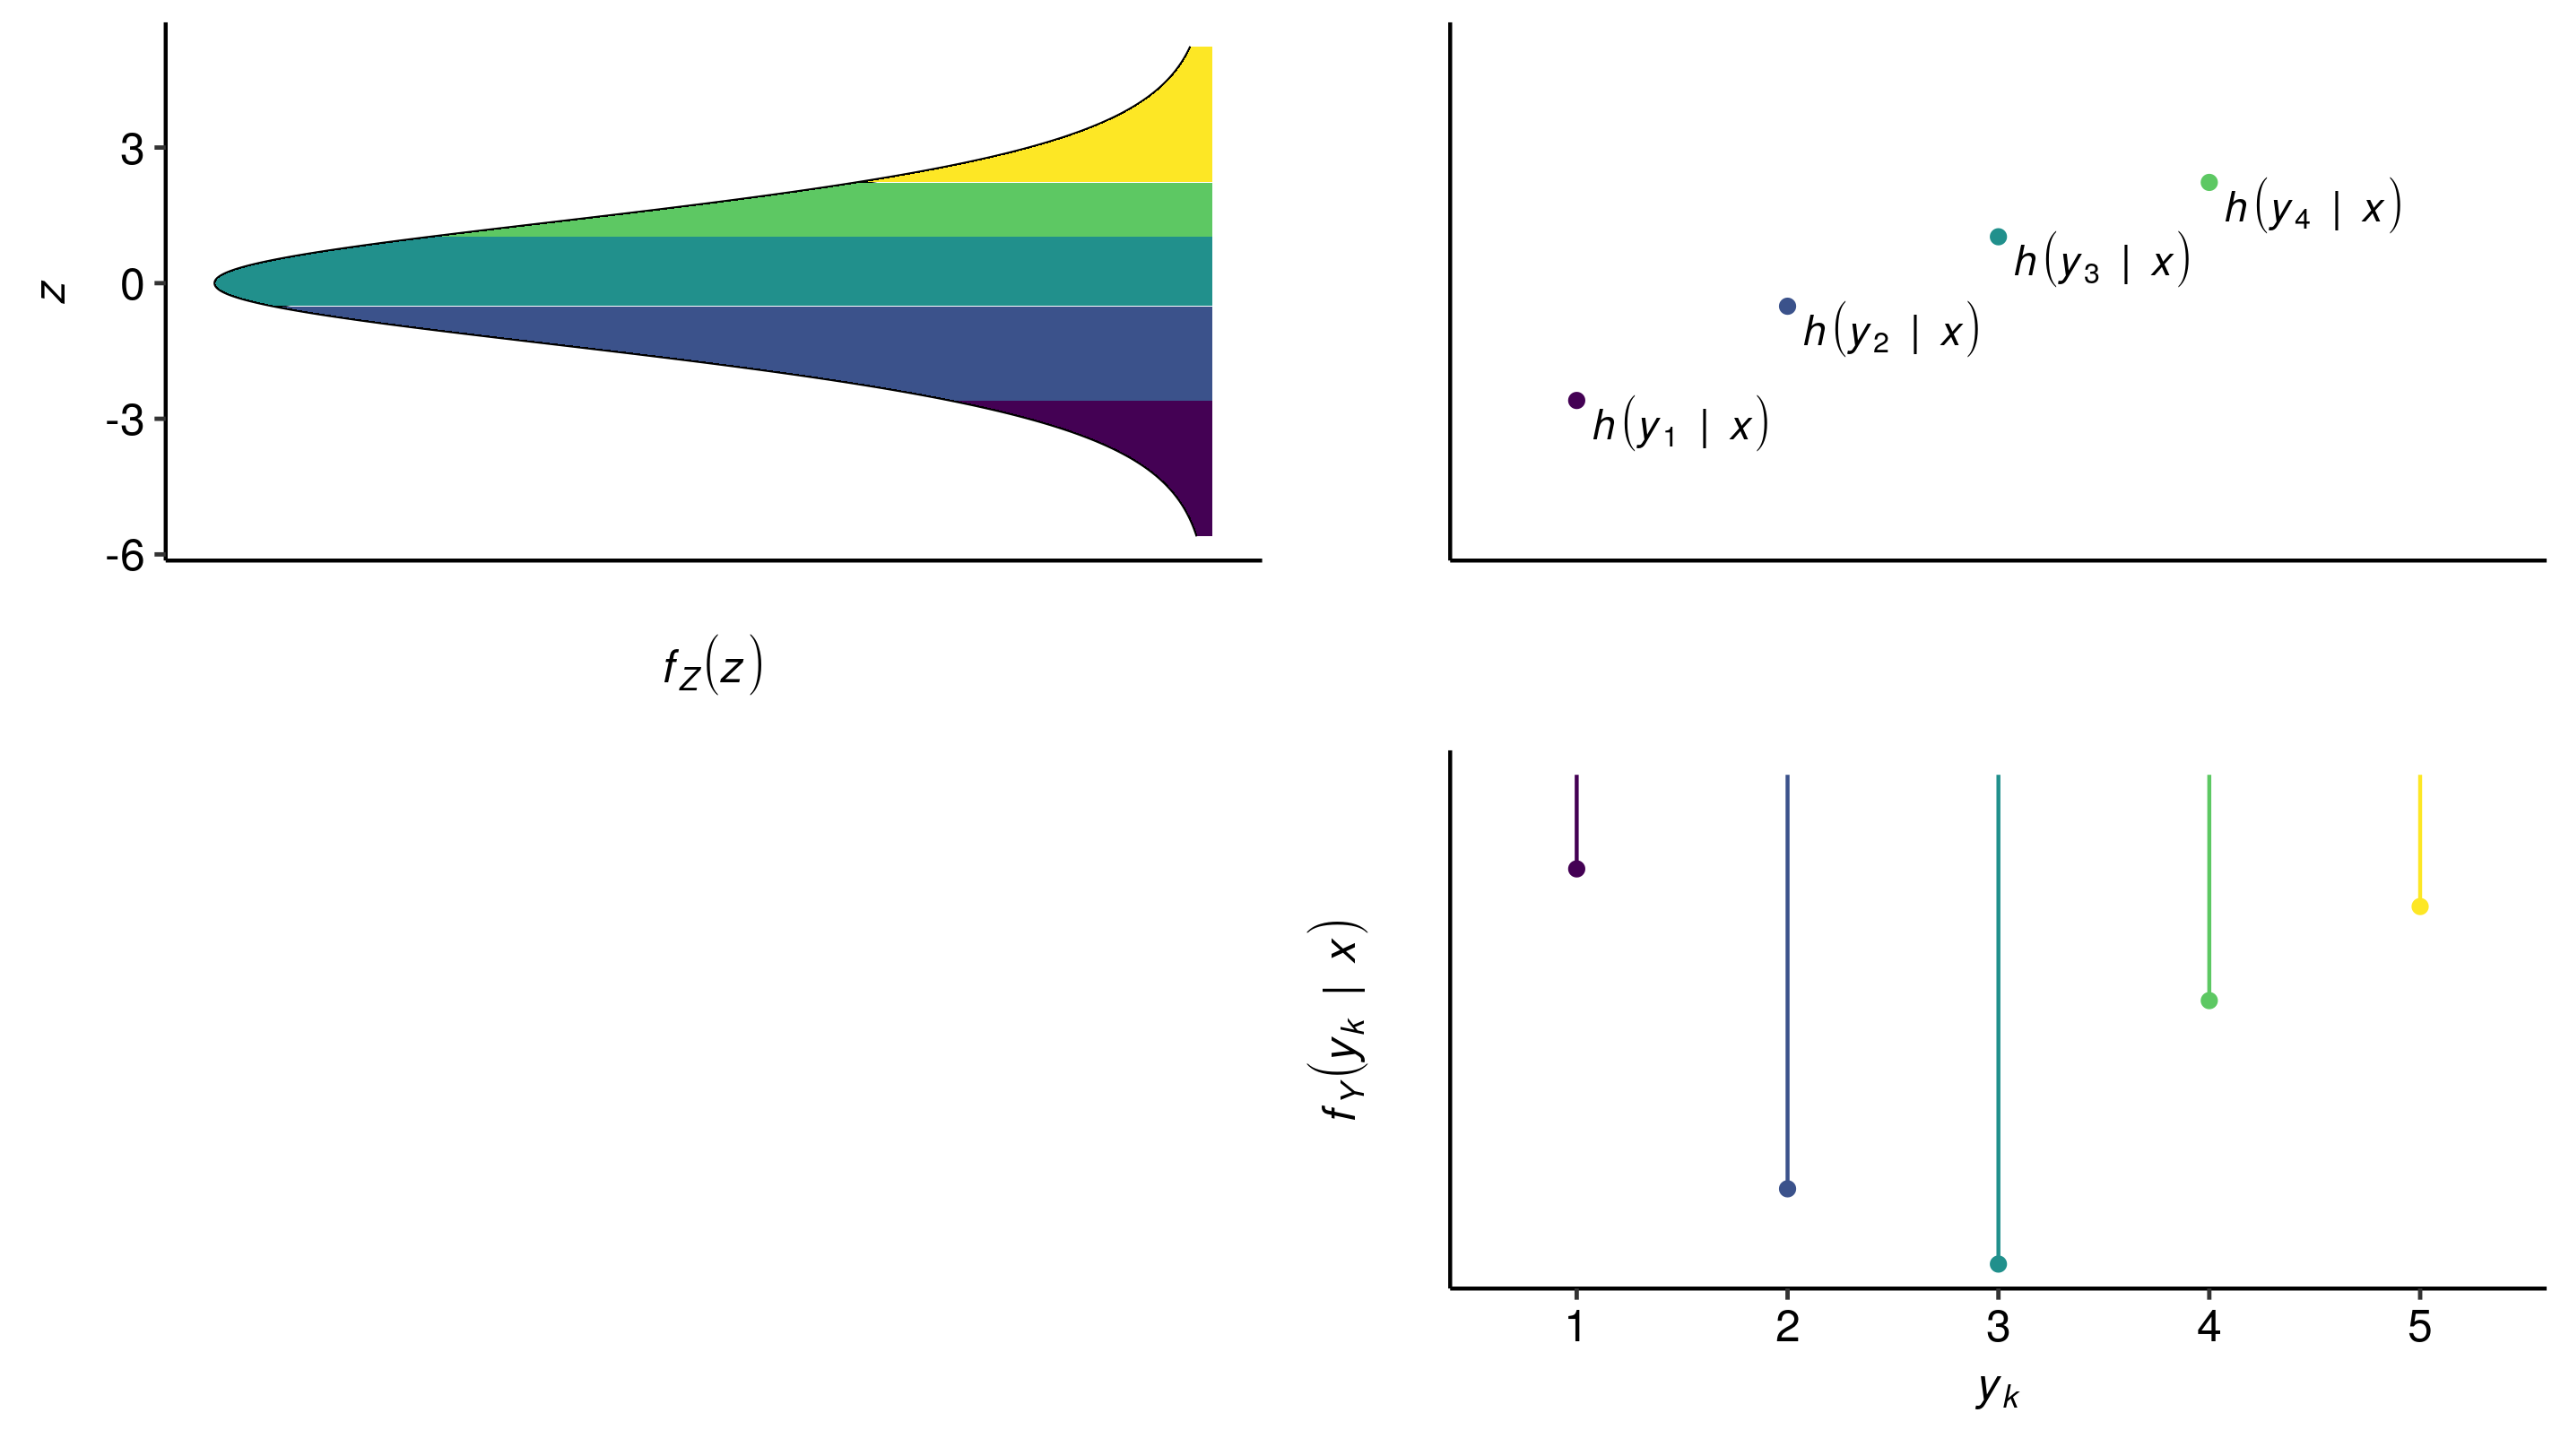
\includegraphics[width=0.8\textwidth]{figures/discrete}
\caption{Illustrating transformation model likelihoods for unconditional ordinal
models. The lower panel shows the unconditional density of $\rY$, which gets
mapped onto the density of $F$ (upper left panel) via the transformation function
(upper right panel). The likelihood contributions are in fact probabilities and
given by the area under the density of $F$ between two consecutive intercepts in the
transformation function. Note that $\eparm_k = + \infty$ does not show on the
plot for the transformation function, but is evident by the yellow area under
the density of $F$.} \label{fig:discrete}
\end{figure}

Deep neural networks gained enormous popularity over the last two decades and
achieved outstanding performances on tasks like natural language processing,
image-based classification problems and many others \citep{goodfellow2016deep}.
Ordinal regression problems come up in a multitude of clinical applications, where
imaging and further clinical data is available.
Ordinary proportional odds models fall short of being applicable to such complex
tasks. They may, hoewever, be extended to include imaging data together with tabular
data via deep neural networks. In the next section we review the concurrent
literature that tackles ordinal regression problems with deep neural networks.
In Section~\ref{sec:contrib} we outline and motivate our contribution of ordinal
neural transformation (\code{ontram}) models, which unite classical statistical
regression models with deep neural networks. In Section~\ref{sec:methods}
\code{ontram} models are described in more detail.

%%%%%%%%%%%%%%%%%%%%%%%%%%%%%%%%%%%%%%%%%%%%%%%%%%%%%%%%%%%%%%%%%%%%%%%%%%%%%%%%
\section{Related work} \label{sec:related}
%-------------------------------------------------------------------------------

\citet{vargas2020cumulative} concisely summarize recent approaches to tackle
ordinal regression problems with deep learning methods, which range from using
an ordinal metric for the evaluation of multi-class classification models to % also cite Alali / look for another?
the construction of novel ordinal loss functions. % cite de la Torre here alreday?
% Pick up again in discussion
The earliest approaches seized the equivalence of an ordinal regression problem
to the $K - 1$ binary sub problems given by $\1(\rY \leq \ry_k), \; k = 1, \dots, K - 1$
\citep{frank2001simple}, which is still being used in applications such as
age estimation \citep{niu2016ordinal, zhu2018facial}. \citet{amorim2018interpreting}
comment on the interpretability of the ensemble neural networks in this $K$-rank % check the name again
approach. % What do they say?
Later, \citet{cheng2008neural} devised a cumulative dummy encoding for the ordinal
response where for $\ry = \ry_k$ we have $\tilde\ry_i = 1$ if $i \leq k$ and $0$
otherwise. Cheng and colleagues then suggest a sigmoid activation for the last
layer of dimension $K$, together with two loss functions (relative entropy and
a squared error loss), which remains highly popular in application
\citep{liu2017ordinal, garg2019robust, cao2019rank, zhu2020ordinal}.
In the meantime the focus shifted towards novel ordinal loss functions involving
Cohen's kappa \citep{cohen1960coefficient, cohen1968weighted, de2018weighted,
de2019deep, vargas2019deep, vargas2020cumulative}, which will be described in
more detail in Section \ref{sec:methods}. \citet{liu2019probabilistic} took
a probabilistic approach using Gaussian processes and an ordinal likelihood
similar to the cumulative probit model.
% Missing: other (more exotic) losses: triplett loss, pixel-wise ordinal loss,
% soft-label loss, SVM loss (can be left out since not DNN?)
% triplett and soft label fits into what Cheng (2008) would call threshold models

Deep transformation models have very recently been applied to
regression problems with a continuous response \citep{sick2020deep}.
Here, the authors parametrized the transformation function as a composition of
linear and sigmoid transformations and a flexible basis expansion that ensures
monotonocity of the resulting transformation function.
% Here, the authors further decomposed the transformation function into an affine
% function followed by a sigmoid transformation, followed by a basis expansion that
% ensures monotonicity and a last affine transformation.
The authors applied deep transformation models to a multitude of data sets with
a continuous response.
However, also the \code{wine} data set was considered, where Sick and colleagues
treated a truly ordinal response as continuous; as did all the other benchmark models.
Again, this is symptomatic for the lack of deep learning models for ordered categorical
data.

%%%%%%%%%%%%%%%%%%%%%%%%%%%%%%%%%%%%%%%%%%%%%%%%%%%%%%%%%%%%%%%%%%%%%%%%%%%%%%%%
\section{Our contribution} \label{sec:contrib}
%-------------------------------------------------------------------------------

In this paper we introduce ordinal neural transformation (\code{ontram}) models
together with a log-likelihood loss which takes the response's natural ordering
into account.

Ordinal regression problems are oftentimes solely viewed as classification problems
with no interest in estimating the underlying conditional distribution.
As such, deep neural networks are trained or evaluated using ordinal loss functions
that do not penalize overly confident predictions.
On the contrary, they may even encourage these overly confident predictions
\citep{brocker2007scoring}.
We thus advocate a framework in which the focus lies on estimating a whole
conditional distribution where estimation and evaluation take place in the
same maximum likelihood-based framework. We want to advocate the use
of proper scoring rules to evaluate test performance of our models, as they
encourage honest predictions of conditional probability distributions
\citep{gneiting2007strictly}.

The goal of \code{ontram} models is to estimate a flexible conditional distribution
while keeping parts of the model interpretable. In many clinical applications
we face ordinal regression tasks based on imaging and tabular clinical data.
Our approach is able to seamlessly integrate imaging and tabular data with
varyingly complex interactions between the two, by taking a modular approach to
model building. The user chooses the interpretational scale to work on by
specifying the inverse cumulative link function $F$ and the complexity of the
transformation function $\h$. The latter will be parametrized by at most three
(deep) neural networks for the intercept function, tabular and image data.
Together with $F$, the output of these three networks will be used to build the
log-likelihood loss. In the end, the model is fit by stochastic gradient descent.

We compare our implementation of ordinal neural transformation models against
a softmax classifier with either categorical cross-entropy or a quadratic weighted
kappa (QWK) loss.
We consider age estimation from facial images and disease grading in diabetic
retinopathy images as applications for our models and discuss the advantages and
limitations of all presented models.
We emphasize interpretability of the different model components and inspect the
loss in performance owed to making the models less flexible.
We furthermore show that the parametrization of the log-likelihood as an ordinal
loss speeds up learning compared to the conventional softmax classifier, even
though the underlying likelihood functions are equivalent up to the mentioned
reparametrization.
% Maybe include wine as well and show that we get on-par performance with
% Sick et al. (2020), where the response is treated as continuous?
% Also include the gain of including clinical covariates / images or vice versa
% Discuss!

%%%%%%%%%%%%%%%%%%%%%%%%%%%%%%%%%%%%%%%%%%%%%%%%%%%%%%%%%%%%%%%%%%%%%%%%%%%%%%%%
\section{Methods} \label{sec:methods}
%-------------------------------------------------------------------------------

Before introducing ordinal neural transformation models, we will describe
multi-class classification (multinomial regression) using softmax as the last
layer activation together with a categorical cross-entropy loss \citep{goodfellow2016deep}.
In addition, we consider an approach to ordinal regression based on the QWK loss
introduced by \citet{de2018weighted}.

\subsection{Multinomial regression} \label{sec:softmax}

In a standard multi-class classification problem the last layer activation is usually
softmax with the output dimension being equal to the number of classes in the
problem. The softmax function is defined as
\begin{align*}
  \softmax(z_k) = \frac{\exp(z_k)}{\sum_{i=1}^K \exp(z_i)},
\end{align*}
where $z_k$ denotes the output of unit $k$.
The function normalizes the outputs to sum to 1, which allows individual components
to be interpretable as probabilities. % Maybe unnecessary to go into too much detail?
% Note that also in multinomial regression settings one is predicting a conditional
% probability distribution. % Somehow make the point here to use scoring rules?
To fit the model, typically the categorical cross-entropy loss is used, which is
equivalent to the multinomial log-likelihood and given by
\begin{align*}
  L(p; y) = - \sum_{k=1}^K y_k \log p(y_k),
\end{align*}
where $p$ denotes the predicted probability distribution.
The categorical-cross-entropy does not take the response's ordering into account,
because it penalizes each misclassification the same way. Yet when dealing with
a categorical response, a misclassification further away from the true class
should yield an appropriately higher penalty.

\subsection{Ordinal regression using the QWK loss} \label{sec:qwk}

The QWK loss is based on Cohen's kappa, which assesses inter-rater agreement and
corrects it for the expected number of agreements under independence, while
taking into account the marginal distributions \citep{cohen1960coefficient}.
Introducing a weighting scheme allows one to penalize predictions far away from
the true label more or less strictly \citep{cohen1968weighted}.
Because Cohen's kappa takes into account the ordinal nature of the response when
weighted accordingly it has been proposed and used as a loss function for deep
ordinal regression problems
\citep{de2018weighted, de2019deep, vargas2019deep, vargas2020cumulative}.
The QWK loss is defined as
\begin{align*}
  L(p) = \log(1 - \kappa(p)),
\end{align*}
where $p$ is the predicted probability distribution and $\kappa$ denotes the
quadratically weighted Cohen's kappa.
Originally defined for count data, \citet{de2018weighted} generalized $\kappa$
to be computable from a probability density.
Because the argument is a conditional probability density, the last layer
activation in a deep neural network can yet again be softmax.

However, the QWK loss is an improper scoring rule and thus encourages dishonest
predictions (\emph{cf.} Appendix \ref{app:improper}).
As such, we emphasize its limited use in estimating conditional distributions
for ordinal outcomes.
However, if one was solely interested in ordinal classification the QWK loss would be
useful to penalize misclassifications farther away from the true label, where the weighting
scheme controls the amount of penalization. % Maybe better suited for the discussion?

\subsection{Ordinal neural transformation models} \label{sec:ontram}

Our approach to deep ordinal regression allows various interpretational scales
and flexibility of model components and is based on maximum likelihood.
Thus, ordinal neural transformation models are highly modular and possess desirable
theoretical properties.
Any transformation model is of the form in Equation \eqref{eq:ctm},
where $F$ induces the interpretational scale of $\h$. The form and flexibility
of the transformation function $\h$ encodes which parts of the full model
are in turn more interpretable or more flexible.
The simplest \code{ontram} model conditioning on tabular data $\rx$ and image
% Simplest, because no interactions are allowed between
% the predictors or between response and predictors in Equation \eqref{eq:simpleontram}
data $\B$ possesses a transformation function
\begin{align} \label{eq:simpleontram}
  \h(\ry_k \given \rx, \B) = \eparm_k - \linpred - \eta(\B),
\end{align}
where $\eparm_k$ is the intercept corresponding to class $k$, $\shiftparm$ is the
vector of coefficients of a single layer neural network with linear activation function
and $\eta : \RR^{\dim(\B)} \rightarrow \RR$ is a convolutional neural network with
linear last layer activation function.
For $F = \expit$ the individual components of $\shiftparm$ are interpretable as
log-odds ratios \citep{tutz2011regression} (\emph{cf.}~Appendix~\ref{app:interpretation}).
Similarly, the output of $\eta$ is the log-odds of belonging to a higher class,
compared to all lower classes and is common to all class boundaries
(proportional odds assumption).
The intercept function is parametrized as a shallow neural network with linear
last layer activation and outputs $\gamma_1, \dots, \gamma_{K-1}$.
In a post-processing step, it is ensured that the transformation function is
non-decreasing via
\begin{align} \label{eq:constr}
  \begin{split}
  \eparm_k = \eparm_1 + \sum_{i = 2}^k \exp(\gamma_i), \quad k \geq 2, \\
  \eparm_0 = - \infty, \; \eparm_1 = \gamma_1, \; \eparm_K = + \infty.
  \end{split}
\end{align}
The resulting vector of intercepts will be denoted $\parm \in \RR^{K + 1}$.
The addition of $\eparm_0$ and $\eparm_K$ as negative and positive infinity
will become apparent when computing the loss.
Enforcing the inequality constraints, in what \citet{cheng2008neural} call
threshold models, has been done similarly in the literature where $\gamma_i$
gets squared instead of exponentiated to ensure the intercept function is
non-decreasing \citep{liu2019probabilistic, vargas2020cumulative}.

Conceptually one is not bound to use a linear predictor for the tabular
data. The above model can be made more flexible, yet less interpretable, by
substituting the linear predictor for a more complex neural network
$\beta : \RR^{\dim(\rx)} \rightarrow \RR$,
\begin{align*}
  \h(\ry_k \given \rx, \B) = \eparm_k - \beta(\rx) - \eta(\B),
\end{align*}
where $\beta(\rx)$ is now a log odds ratio function that allows for higher order
interactions between all $p$ predictors.
Another layer of complexity can be added by allowing the intercept function
$\eparm_k$ for $\ry = \ry_k$, to depend on the image
\begin{align*}
  \h(\ry_k \given \rx, \B) = \eparm_k(\B) - \beta(\rx),
\end{align*}
which can be achieved using a convolutional neural network with linear last
layer activation and $K - 1$ output nodes. Its output will be processed
equivalently to the simple intercept function in \eqref{eq:constr}, now
for every image.
Here, we speak of response-varying effects, as the intercept function
(a function of the response) is now allowed to vary with the image \citep{hothorn2018most}.
% Stress how this works, and that we're the first to do use threshold models
% with rv effects

One does not necessarily have to stop here. Including both the image and
the tabular data as response-varying effects
\begin{align*}
  \h(\ry_k \given \rx, \B) = \eparm_k(\rx, \B),
\end{align*}
further increases model complexity while decreasing interpretability.
This model is in fact equivalent to using softmax as the last layer activation
and a categorical crossentropy loss, albeit parametrized differently
\citep{hothorn2014conditional}.
The tabular data may be attached to the feature vector resulting from the
convolutional part of a convolutional neural network.
Single model components may also be omitted such that the model depends on image
or tabular data only. This high modularity enables many more applications of
\code{ontram} models.

The loss function for \code{ontram} models is based on the transformation model
log-likelihood. For the model in \eqref{eq:simpleontram} a single log-likelihood
contribution is given by
\begin{align*}
  \ell(\parm, \shiftparm, \eta ; \ry_k, \rx, \B)
  &= \log\prob(\rY = \ry_k \given \rx, \B) \\
  &= \log\left(\prob(\rY \leq \ry_k \given \rx, \B) - \prob(\rY \leq \ry_{k-1} \given \rx, \B)\right) \\
  &= \log\left(F\left(\eparm_k - \linpred - \eta(\B)\right) -
    F\left(\eparm_{k-1} - \linpred - \eta(\B)\right)\right).
\end{align*}
In its most general form one can write the \code{ontram} loss as
\begin{align*}
  \ell(\h ; \ry_k, \rx, \B) = \log\left(F(\h(\ry_k \given \rx, \B)\right) -
    F\left(\h(\ry_{k-1} \given \rx, \B)\right)), \; k = 1, \dots, K,
\end{align*}
which encompasses all the models in Table \ref{tab:mods}.
Note that for $k = 1$ and $k = K$ we have
\begin{align*}
  &\log\left(F\left(\eparm_1 - \linpred - \eta(\B)\right) -
    F\left(\eparm_{0} - \linpred - \eta(\B)\right)\right)
    = \log\left(F\left(\eparm_1 - \linpred - \eta(\B)\right)\right) \mbox{ and} \\
  &\log\left(F\left(\eparm_K - \linpred - \eta(\B)\right) -
    F\left(\eparm_{K-1} - \linpred - \eta(\B)\right)\right)
    = \log\left(1 - F\left(\eparm_{K-1} - \linpred - \eta(\B)\right)\right),
\end{align*}
respectively, because $\eparm_0 = - \infty$ and $\eparm_K = + \infty$.

\begin{figure}
\centering
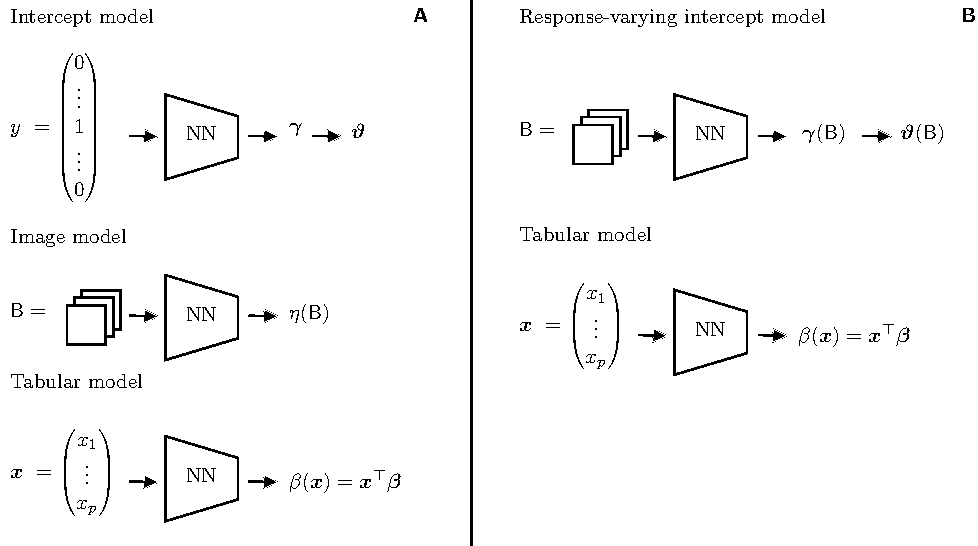
\includegraphics[width=1\textwidth]{figures/ontram-architecture}
\caption{Model architecture for the complex shift (A) and response-varying (B)
\code{ontram} models.} \label{fig:ontram}
\end{figure}

\begin{figure}
\centering
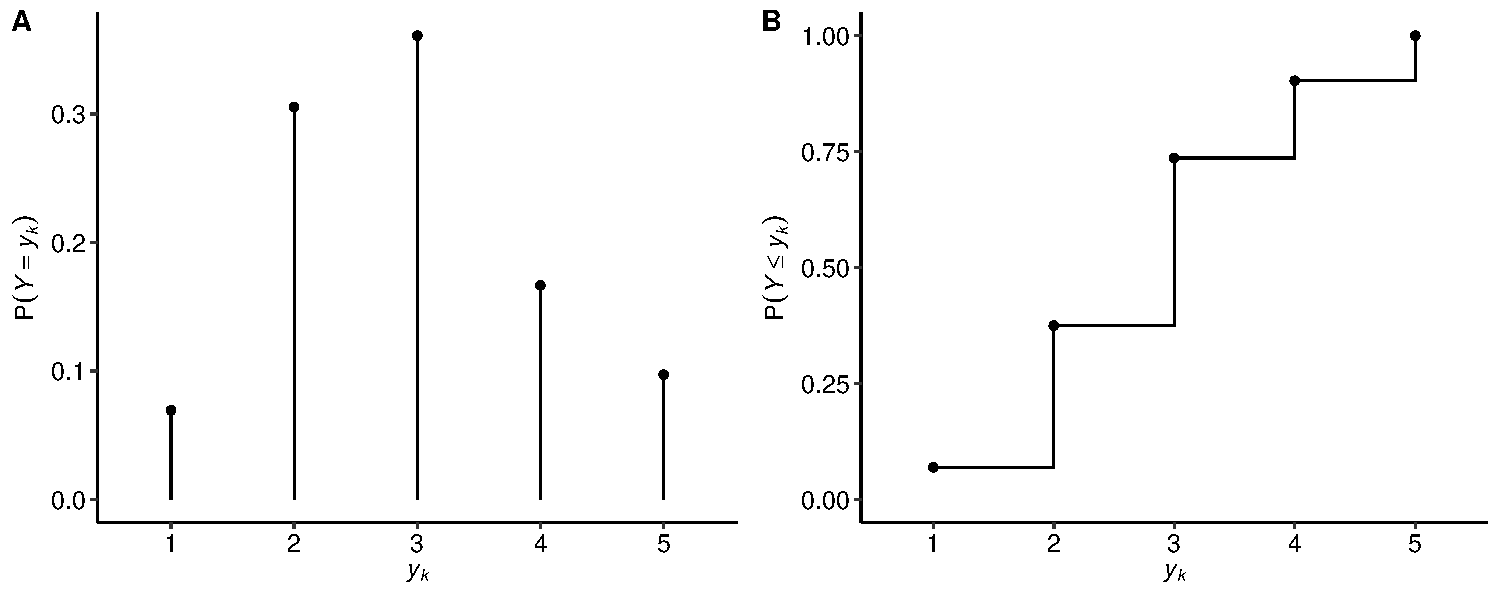
\includegraphics[width=1\textwidth]{figures/figure0}
\caption{Density (A) and cumulative distribution (B) of an ordinal random
variable} \label{fig:ordinal}
\end{figure}

\begin{figure}
\centering
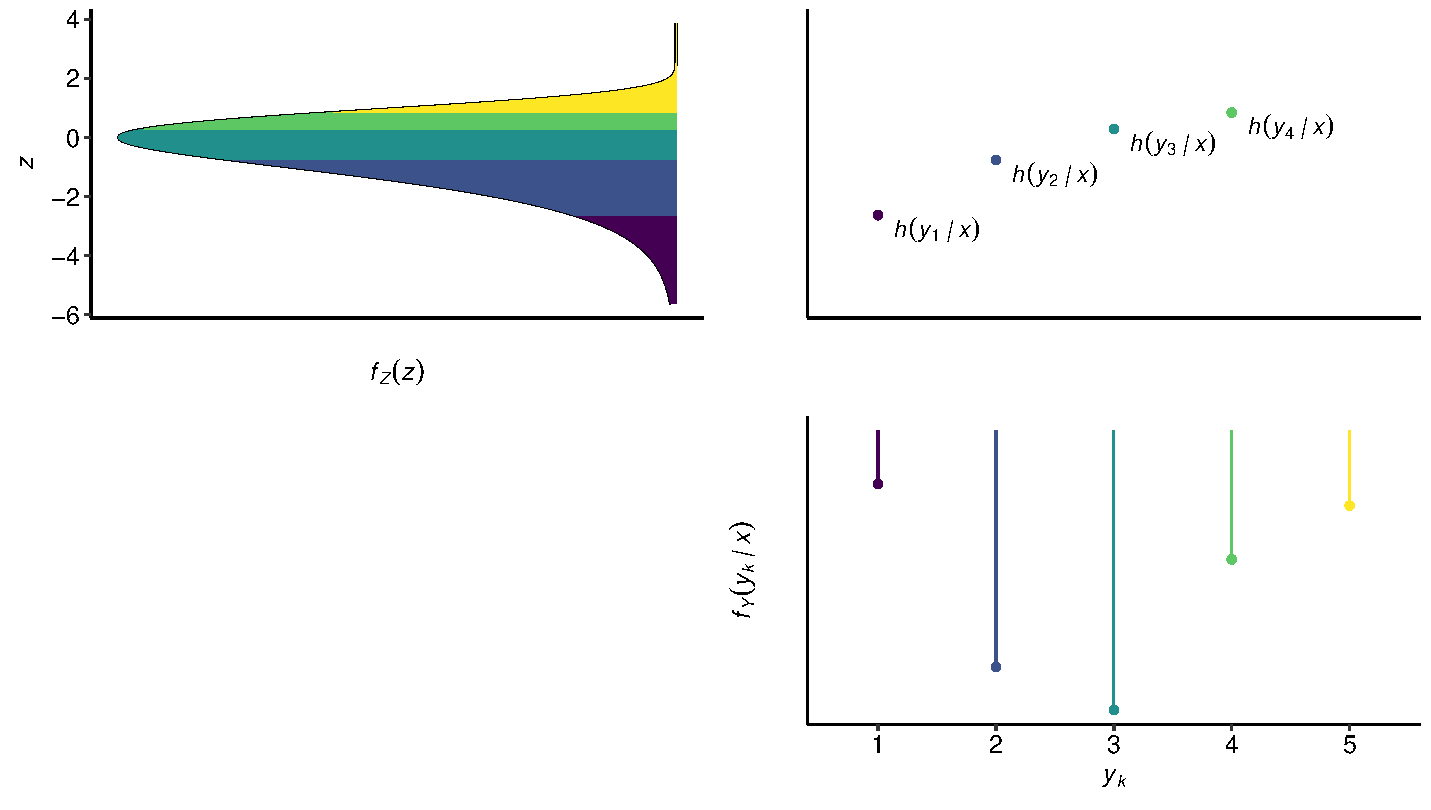
\includegraphics[width=0.8\textwidth]{figures/discrete-cloglog}
\caption{Same as Figure~\ref{fig:discrete}, but with $F=\pMEV$. The density of the
standard minimum extreme value distribution is skewed, which the transformation
function takes into account, such that the resulting unconditional density is the
same as in Figure~\ref{fig:discrete}. Thus, unconditional ordinal transformation
models are invariant w.r.t. the choice of $F$ and always produce the same
distribution by adapting the transformation function.} \label{fig:discrete-cloglog}
\end{figure}

\begin{figure}
\centering
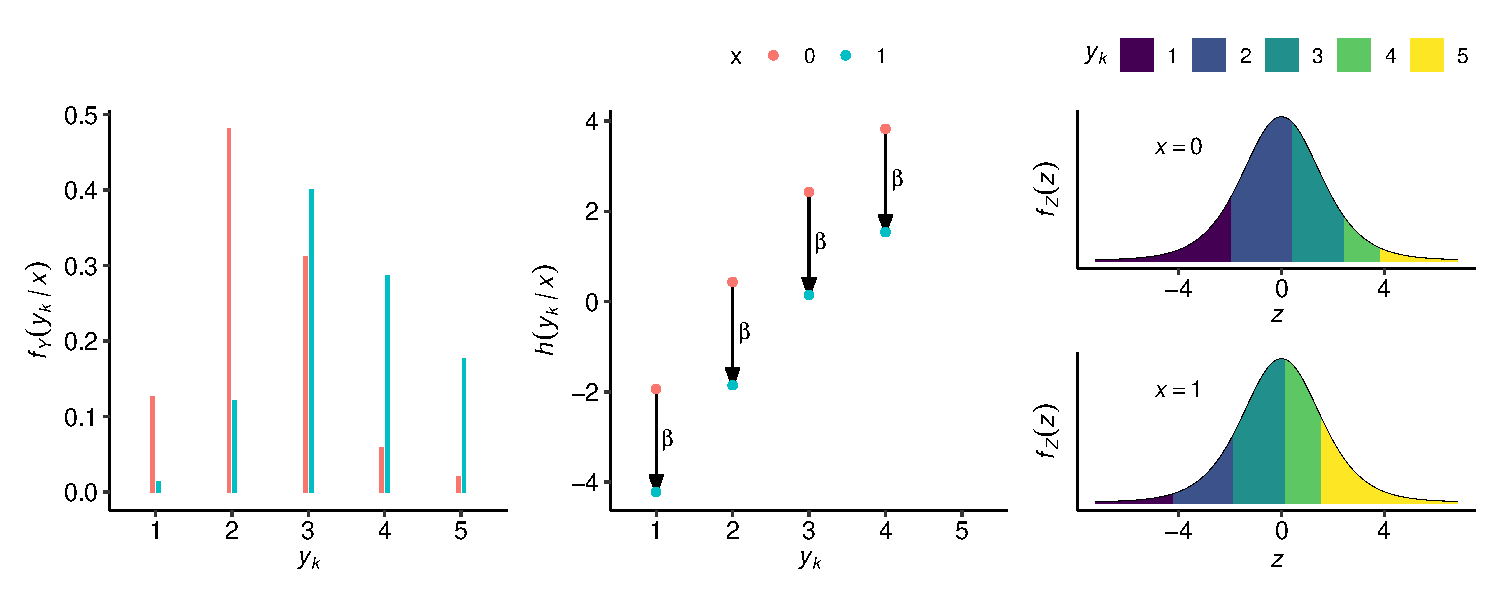
\includegraphics[width=1\textwidth]{figures/conditional-polr}
\caption{Illustrating the effect of linear predictors on likelihood (left),
transformation (middle) and density function (right) in a POLR model.
The transformation function shifts downwards by $\linpred$, which in turn changes
the shape of the cdf and the corresponding likelihood contributions as areas under
the density of $F$.} \label{fig:cpolr}
\end{figure}

\begin{figure}
\centering
\begin{tikzpicture}[auto, Arr/.style={-{Latex[length=1.5mm]}}]
  \node (X2) {$X_2$};
  \node [below =1.5cm of X2] (X3) {$X_3$};
  \node (Xn) [below =1.5cm of X3] {$X_{\{1, 4, 7, 8, 9, 10\}}$};
  \node [below =1.5cm of Xn] (X5) {$X_5$};
  \node [below =1.5cm of X5] (X6) {$X_6$};
  \node [right =8cm of Xn] (Y) {$Y$};
  \node [right =3cm of Y] (B) {$\B$};
  \draw[Arr] (X2) to [bend left=20, "$+ \log 1.2$"] (Y);
  \draw[Arr] (X3) to [bend left=20, "$- \log 1.2$"] (Y);
  \draw[Arr] (Xn) to ["$0$"] (Y);
  \draw[Arr] (X5) to [bend right=20, "$+ \log 1.5$"] (Y);
  \draw[Arr] (X6) to [bend right=20, "$- \log 1.5$"] (Y);
  \draw[Arr, dotted] (B) to (Y);
\end{tikzpicture}
\caption{Simulation of predictors for UTKFace and DR data. $X_j \sim \ND(0, \sigma^2)$,
$j = 1, \dots, 10$, with $\sigma = 1.55$ for UTKFace and $\sigma = 1.4$ for DR.
The predictors $X_j$ are simulated under a proportionality assumption. That is,
the effect of $\shiftparm$ is common to all class boundaries. Note that the arrows
indicate effects on the log-odds scale of the outcome $\rY$, i.e.,
$\pY(\ry_k \given \rx) = F_L(\eparm_k - \linpred)$.} \label{fig:sim}
\end{figure}

%%%%%%%%%%%%%%%%%%%%%%%%%%%%%%%%%%%%%%%%%%%%%%%%%%%%%%%%%%%%%%%%%%%%%%%%%%%%%%%%
\section{Experiments} \label{sec:experiments}
%-------------------------------------------------------------------------------

\subsection{Datasets}

\code{Wine quality:} The \code{wine quality} dataset consists of 4898 observations of wine
quality measured on an ordinal scale with 10 levels of which only 6 were observed.
Additionally, the dataset contains 11 other covariates, such as acidity, citric acid and
sugar content \citep{cortez2009modeling}.
We employ the same cross-validation scheme as \citet{gal2015dropout}, who used a
subset of the data (red wine, $n = 1599$) and split the data into 20 folds of
90\% training and 10\% test data.

\subsection{Neural network architectures}

\emph{Wine quality}: The wine quality data was modeled using a densely connected
neural network with four layers with 16 units each. Between layers 1, 2, and 3, we
specified a dropout layer with dropout rate 0.3. Architectures for the different
models only differ in their last layer and its corresponding activation function.
The baseline (BL) and quadratic weighted kappa (qwk) models end with a 5-dimensional
softmax layer and the response varying ontram model (rv) in a 4-dimensional linear
layer to encode the raw intercept parameters of the transformation function.
The complex shift (cs) model possesses the same architecture as the above models
and ends in a 1-unit linear activation.
The simplest model, proportional odds logistic regression (polr), contains only a
linear predictor to model the covariate shifts (that is, a one layer NN with linear
activation and no bias). We compared the polr model to the implementation in the
\proglang{R}-addon package \pkg{tram} \citep{pkg:tram}.

\subsection{Evaluation procedures}

\emph{Wine quality}:
The data set was split into 20 cross-validation folds of 90\% train and 10\% test data.
The predictors were scaled to have mean zero and unit variance.
Otherwise, no further preprocessing was undertaken.
All models were trained via stochastic gradient descent using a learning rate of
0.001.
All models, except for qwk, were trained for 100 epochs with a batch size of 6.
The qwk model was trained for 1000 epochs with a batch size of 1599, because the
QWK loss and its gradient become more stable for larger batch sizes \citep{de2018weighted}.
Otherwise, no further fine tuning of the models was done.
Evaluation metrics included categorical cross-entropy, the QWK loss transformed
back to its original scale, the discrete quadratic weighted kappa as computed from
the confusion matrix, and accuracy.

\subsection{Models}

Performance of the ontram models is assessed using six different models with
image data and a combination of image and patient data as inputs (Table~\ref{tab:mods}).

\begin{table}
\centering
\caption{Models used throughout the paper. $D$ denotes the data used for the model which
in our applications would be $D \in \calD = 2^{\{\rx, \B\}}$.
Here, $2^A$ denotes the power set of $A$.} \label{tab:mods}
\begin{tabular}{@{}llll@{}}
\toprule
\textbf{Experiment}
& \textbf{Name}                   & \textbf{Abbreviation} & \textbf{Trafo} $\h(\ry \given D)$ \\ \midrule
\multirow{5}{*}{Wine}
& Multiclass classification       & MCC                   &                \\
& QWK loss                        & QWK                   &                \\ \cline{2-4}
& Complex intercept               & CI$_x$                &  $\eparm_k(\rx)$ \\
& Simple intercept + complex shift& SI-CS$_x$             &  $\eparm_k - \beta(\rx)$ \\
& Simple intercept + linear shift & SI-LS$_x$             &  $\eparm_k - \linpred$ \\ \midrule
\multirow{8}{*}{DR \& Face}
& Multiclass classification       & MCC                   &                \\
& Multiclass classification + tabular& MCC-$x$            &                \\
& QWK loss                        & QWK                   &                \\
& QWK loss + tabular              & QWK-$x$               &                \\ \cline{2-4}
& Complex intercept               & CI$_\B$               & $\eparm_k(\B)$ \\
& Complex intercept + tabular     & CI$_\B$-LS$_x$        & $\eparm_k(\B) - \linpred$ \\
& Simple intercept + complex shift& SI-CS$_\B$            & $\eparm_k - \eta(\B)$ \\
& Simple intercept + complex shift + tabular& SI-CS$_\B$-LS$_x$ & $\eparm_k - \eta(\B) - \linpred$ \\ \bottomrule
\end{tabular}
\end{table}

%%%%%%%%%%%%%%%%%%%%%%%%%%%%%%%%%%%%%%%%%%%%%%%%%%%%%%%%%%%%%%%%%%%%%%%%%%%%%%%%
\section{Results} \label{sec:results}
%-------------------------------------------------------------------------------

\code{Wine quality:}
All three \code{ontram} models achieve comparable performance to the most flexible
softmax model in terms of categorical cross-entropy (\emph{cf.} Figure~\ref{fig:res:wine}).
Taking the ordering into account, however, the response-varying and complex shift
\code{ontram} models achieve a better quadratic weighted kappa and QWK loss.
The qwk model outperforms all other models in terms of QWK loss and quadratic
weighted kappa on average, while showing the worst categorical cross-entropy
across all folds. Additionally, the qwk model has the poorest accuracy on average.
The qwk model's poor performance in terms of categorical cross-entropy and the
fact that both QWK and discrete QWK are so similar can be traced back to the
impropriety of the QWK loss. The QWK loss encourages overconfident predictions,
thus putting almost all probability mass on the mode of the predicted distribution.
This, in turn, leads to the same kappa.

The gain in performance by using the more complex response-varying model is almost
negligible compared to the complex shift model, the latter of which possesses a
higher degree of interpretability. At the same time the simple polr model may
be too inflexible achieving a QWK and accuracy comparable only to the softmax model,
albeit much easier to interpret.

Although polr and t-polr are completely equivalent models, the stochastic nature
of fitting the \code{ontram} polr model reflects in a slightly weaker performance
across all four metrics when compared to \pkg{tram}'s implementation of the polr
model. Achieving complete equivalence in terms of likelihood and estimated coefficients
requires more careful tuning of batch size, epochs and learning rate.

\begin{figure}
\centering
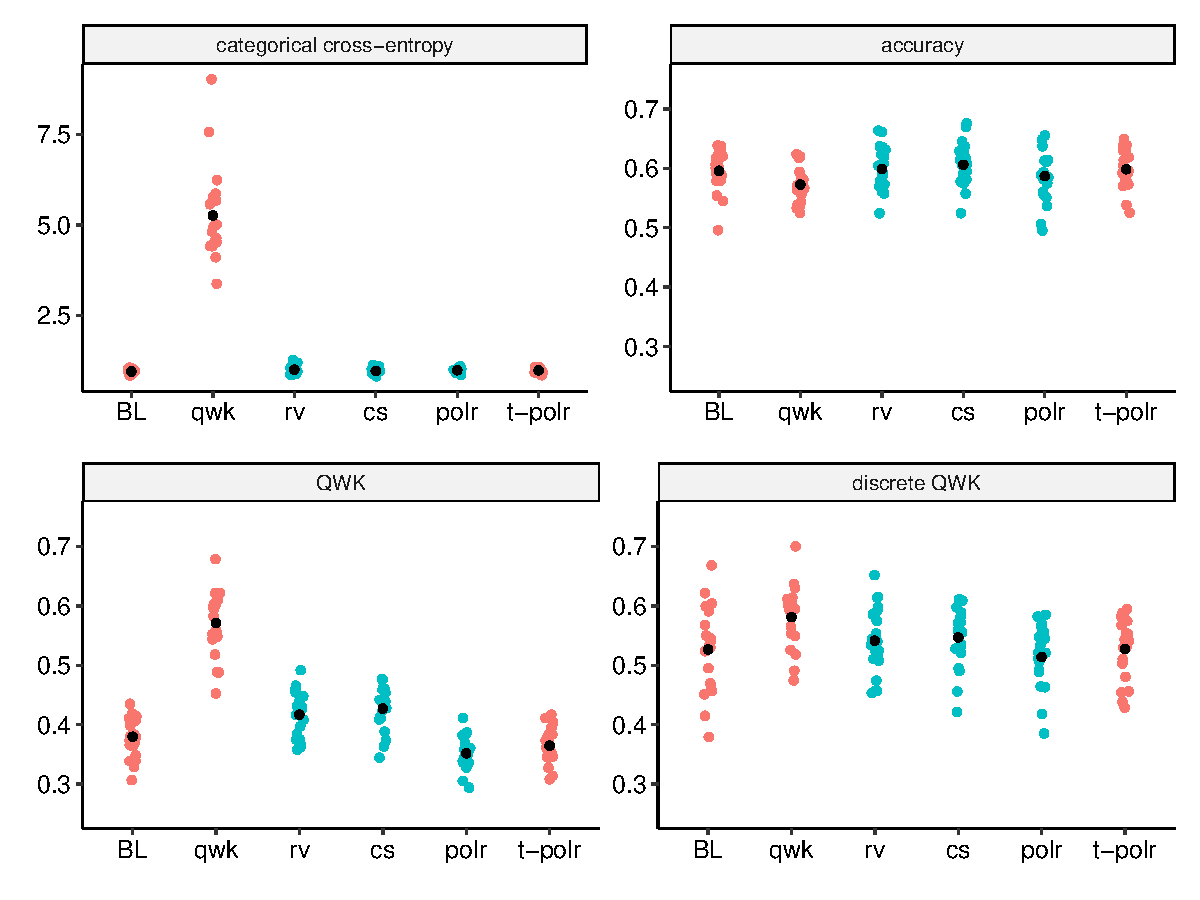
\includegraphics[width=1\textwidth]{figures/wine_test_metric}
\caption{Test performance on the \code{wine quality} data set over 20 cross-validation
folds. Categorical cross-entropy, quadratic weighted kappa computed from the
QWK loss function, discrete quadratic weighted kappa computed from the confusion
matrix and accuracy are displayed for several models. \code{ontram} models are
colored in blue and black dots indicate the mean metric.
The polr and t-polr models contain only a linear predictor and were fit via
stochastic gradient descent and constrained convex optimization, respectively.
\textsf{BL} = last-layer softmax with categorical cross-entropy loss,
\textsf{qwk} = last-layer softmax with QWK loss, \textsf{rv} = \code{ontram}
with response-varying effects, \textsf{cs} = \code{ontram} with complex shift effects,
\textsf{polr} = \code{ontram} with simple shift effects, \textsf{t-polr} = \pkg{tram}
implementation of a proportional odds logistic regression model.} \label{fig:res:wine}
\end{figure}


%%%%%%%%%%%%%%%%%%%%%%%%%%%%%%%%%%%%%%%%%%%%%%%%%%%%%%%%%%%%%%%%%%%%%%%%%%%%%%%%
\section{Discussion} \label{sec:discussion}
%-------------------------------------------------------------------------------

\clearpage

\begin{appendix}
%%%%%%%%%%%%%%%%%%%%%%%%%%%%%%%%%%%%%%%%%%%%%%%%%%%%%%%%%%%%%%%%%%%%%%%%%%%%%%%%
\section{Impropriety of the QWK loss} \label{app:improper}
%-------------------------------------------------------------------------------

\citet{brocker2007scoring} stress the importance of proper scoring rules for
honest distributional forecasts.
A proper score $S$ for any two probability densities $p$ and $q$ fulfills
\begin{align*}
  \Ex_q[S(q, y)] \leq \Ex_q[S(p, y)],
\end{align*}
for any density $p$ and equality holds iff $p = q$ \citep{gneiting2007strictly}.

\citet{de2018weighted} propose a loss function based on the quadratic weighted
kappa \citep{cohen1968weighted} and use it to assess the performance of several
models on test data sets. It is of crucial importance to know, whether the loss
\begin{align*}
  L(p) = \log(1 - \kappa(p))
\end{align*}
is a proper scoring rule, because impropriety encourages dishonest forecasts.

Take the density of an ordinal random variable $Y \in \{y_1 < y_2 < y_3\}$ to be
\begin{align*}
  p(y) =
    \begin{cases}
      0.3 & \mbox{if } y = y_1, \\
      0.4 & \mbox{if } y = y_2, \\
      0.3 & \mbox{if } y = y_3; \\
    \end{cases}
\end{align*}
for which the expected score will be

\begin{align*}
  \Ex_p(\log(1 - \kappa(p))) = \sum_{i = 1}^K p(y_i) \log(1 - \kappa(p))
  = -0.693.
\end{align*}
However, by forecasting a density that puts more mass on $p$'s mode, $y = y_2$,
\begin{align*}
  \tilde{p}(y) =
    \begin{cases}
      0.1 & \mbox{if } y = y_1, \\
      0.8 & \mbox{if } y = y_2, \\
      0.1 & \mbox{if } y = y_3; \\
    \end{cases}
\end{align*}
we can achieve a much lower (better) score
\begin{align*}
  \Ex_{p}(\log(1 - \kappa(\tilde{p}))) = \sum_{i = 1}^K
    p(y_i) \log(1 - \kappa(\tilde{p}))
  = -1.386,
\end{align*}
which proves impropriety of $L$ by counterexample.
The same argument holds for $K = 2$ and $K \geq 3$, as well as different weighting
schemes (no weighting, linear weights, higher order weights).

%%%%%%%%%%%%%%%%%%%%%%%%%%%%%%%%%%%%%%%%%%%%%%%%%%%%%%%%%%%%%%%%%%%%%%%%%%%%%%%%
\section{Interpretational scales} \label{app:interpretation}
%-------------------------------------------------------------------------------

Classical regression textbooks, like \citet{tutz2011regression}, discuss
$F \in \{\expit, \pMEV, \pGumbel, \pN\}$ which are called cumulative logit,
minimum extreme value, maximum extreme value and probit models, respectively.
\citet{tutz2011regression} also derives the interpretational scales and stresses,
that the coefficients resulting from a cumulative probit model are hard to interpret.

For $F = \expit$ we have
\begin{align*}
	\prob(\rY \leq \ry_k \given \rx) &= \expit(\eparm_k - \linpred) \\
	\logit(\prob(\rY \leq \ry_k \given \rx)) &= \eparm_k - \linpred \equiv \omega(\ry_k \given \rx) \\
\end{align*}
Now $\linpred = \omega(\ry_k \given \rx) - \omega(\ry_k \given \rx = 0)$, or on the
odds-scale
\begin{align*}
	\frac{\pY(\ry_k \given \rx)}{1 - \pY(\ry_k \given \rx)} =
		\frac{\pY(\ry_k \given \rx = 0)}{1 - \pY(\ry_k \given \rx = 0)}
		\exp(-\linpred)
\end{align*}
which shows that $\shiftparm$ are interpretable as log odds-ratios. In the same way,
$\eta(\B)$ can be interpreted as a log odds-ratio.

Table~\ref{tab:interpretation} summarizes the four most commonly used cumulative
ordinal regression models and the interpretational scales $F$ induces.

\begin{table}
\centering
\caption{Interpretational scales induced by $F$ \citep{tutz2011regression}.} \label{tab:interpretation}
\begin{tabular}{llll}
\toprule
\textbf{Inverse link} & \textbf{Link} & \textbf{Symbol} &
  \textbf{Interpretation of} $\beta$ \textbf{and} $\eta$ \\ \midrule
Logistic & $\logit$ & $\expit$ & log-odds ratio \\
Gompertz & cloglog & $\pMEV$ & log-hazard ratio \\
Gumbel & loglog & $\pGumbel$ & log-hazard ratio for $\rY_r = K + 1 - \rY$\\
Normal & probit & $\pN$ & not interpretable directly \\
\bottomrule
\end{tabular}
\end{table}

%%%%%%%%%%%%%%%%%%%%%%%%%%%%%%%%%%%%%%%%%%%%%%%%%%%%%%%%%%%%%%%%%%%%%%%%%%%%%%%%
\section{Learning speed under permuted class labels} \label{app:permute}
%-------------------------------------------------------------------------------

In contrast to softmax models with categorical cross-entropy loss, \code{ontram}
models take the response's ordering into account.
This is reflected in the learning curve when comparing \code{ontram} to softmax
models (\emph{cf.} Figure~\ref{fig:permcs}).
When fitting the model on the true ordering the complex shift model outperforms
the softmax model in terms of learning speed and loss, although the model is
much less complex.
Permuting the order does not affect the learning curves of the softmax model.
However, complex shift model underperforms in the presence of wrongly ordered
categories in learning speed and loss compared to the softmax model.

\begin{figure}
\centering
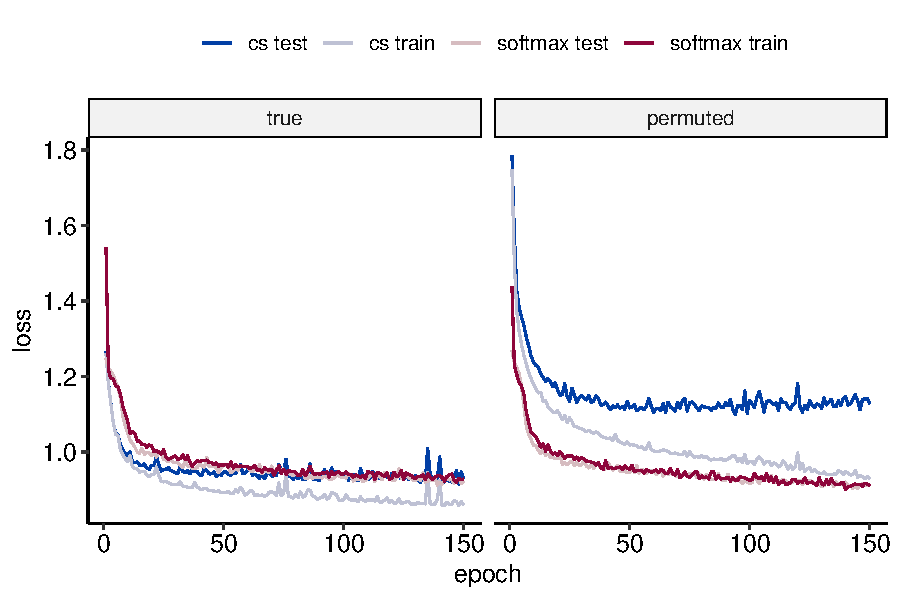
\includegraphics[width=1\textwidth]{figures/permuted-labels-cs}
\caption{Sensitivity to permuted labels for \code{ontram} complex shift models.
Learning curves for train and test loss on the \code{wine quality} data set.
\code{ontram} models take ordering into account and benefit from the similarity
between consecutive classes, explaining their poor performance under permuted
labels. In contrast, the softmax model ignores the ordering and learns equally
well under permuted classes.} \label{fig:permcs}
\end{figure}
\end{appendix}

\clearpage

\bibliography{bibliography,packages}





\end{document}
